
%% bare_conf.tex
%% V1.3
%% 2007/01/11
%% by Michael Shell
%% See:
%% http://www.michaelshell.org/
%% for current contact information.
%%
%% This is a skeleton file demonstrating the use of IEEEtran.cls
%% (requires IEEEtran.cls version 1.7 or later) with an IEEE conference paper.
%%
%% Support sites:
%% http://www.michaelshell.org/tex/ieeetran/
%% http://www.ctan.org/tex-archive/macros/latex/contrib/IEEEtran/
%% and
%% http://www.ieee.org/

%%*************************************************************************
%% Legal Notice:
%% This code is offered as-is without any warranty either expressed or
%% implied; without even the implied warranty of MERCHANTABILITY or
%% FITNESS FOR A PARTICULAR PURPOSE! 
%% User assumes all risk.
%% In no event shall IEEE or any contributor to this code be liable for
%% any damages or losses, including, but not limited to, incidental,
%% consequential, or any other damages, resulting from the use or misuse
%% of any information contained here.
%%
%% All comments are the opinions of their respective authors and are not
%% necessarily endorsed by the IEEE.
%%
%% This work is distributed under the LaTeX Project Public License (LPPL)
%% ( http://www.latex-project.org/ ) version 1.3, and may be freely used,
%% distributed and modified. A copy of the LPPL, version 1.3, is included
%% in the base LaTeX documentation of all distributions of LaTeX released
%% 2003/12/01 or later.
%% Retain all contribution notices and credits.
%% ** Modified files should be clearly indicated as such, including  **
%% ** renaming them and changing author support contact information. **
%%
%% File list of work: IEEEtran.cls, IEEEtran_HOWTO.pdf, bare_adv.tex,
%%                    bare_conf.tex, bare_jrnl.tex, bare_jrnl_compsoc.tex
%%*************************************************************************

% *** Authors should verify (and, if needed, correct) their LaTeX system  ***
% *** with the testflow diagnostic prior to trusting their LaTeX platform ***
% *** with production work. IEEE's font choices can trigger bugs that do  ***
% *** not appear when using other class files.                            ***
% The testflow support page is at:
% http://www.michaelshell.org/tex/testflow/



% Note that the a4paper option is mainly intended so that authors in
% countries using A4 can easily print to A4 and see how their papers will
% look in print - the typesetting of the document will not typically be
% affected with changes in paper size (but the bottom and side margins will).
% Use the testflow package mentioned above to verify correct handling of
% both paper sizes by the user's LaTeX system.
%
% Also note that the "draftcls" or "draftclsnofoot", not "draft", option
% should be used if it is desired that the figures are to be displayed in
% draft mode.
%
\documentclass[conference, ngerman]{IEEEtran}
\usepackage{blindtext, graphicx}
\usepackage[utf8]{inputenc}
\usepackage[ngerman]{babel}

% Add the compsoc option for Computer Society conferences.
%
% If IEEEtran.cls has not been installed into the LaTeX system files,
% manually specify the path to it like:
% \documentclass[conference]{../sty/IEEEtran}





% Some very useful LaTeX packages include:
% (uncomment the ones you want to load)


% *** MISC UTILITY PACKAGES ***
%
%\usepackage{ifpdf}
% Heiko Oberdiek's ifpdf.sty is very useful if you need conditional
% compilation based on whether the output is pdf or dvi.
% usage:
% \ifpdf
%   % pdf code
% \else
%   % dvi code
% \fi
% The latest version of ifpdf.sty can be obtained from:
% http://www.ctan.org/tex-archive/macros/latex/contrib/oberdiek/
% Also, note that IEEEtran.cls V1.7 and later provides a builtin
% \ifCLASSINFOpdf conditional that works the same way.
% When switching from latex to pdflatex and vice-versa, the compiler may
% have to be run twice to clear warning/error messages.






% *** CITATION PACKAGES ***
%
%\usepackage{cite}
% cite.sty was written by Donald Arseneau
% V1.6 and later of IEEEtran pre-defines the format of the cite.sty package
% \cite{} output to follow that of IEEE. Loading the cite package will
% result in citation numbers being automatically sorted and properly
% "compressed/ranged". e.g., [1], [9], [2], [7], [5], [6] without using
% cite.sty will become [1], [2], [5]--[7], [9] using cite.sty. cite.sty's
% \cite will automatically add leading space, if needed. Use cite.sty's
% noadjust option (cite.sty V3.8 and later) if you want to turn this off.
% cite.sty is already installed on most LaTeX systems. Be sure and use
% version 4.0 (2003-05-27) and later if using hyperref.sty. cite.sty does
% not currently provide for hyperlinked citations.
% The latest version can be obtained at:
% http://www.ctan.org/tex-archive/macros/latex/contrib/cite/
% The documentation is contained in the cite.sty file itself.






% *** GRAPHICS RELATED PACKAGES ***
%
\ifCLASSINFOpdf
  % \usepackage[pdftex]{graphicx}
  % declare the path(s) where your graphic files are
  % \graphicspath{{../pdf/}{../jpeg/}}
  % and their extensions so you won't have to specify these with
  % every instance of \includegraphics
  % \DeclareGraphicsExtensions{.pdf,.jpeg,.png}
\else
  % or other class option (dvipsone, dvipdf, if not using dvips). graphicx
  % will default to the driver specified in the system graphics.cfg if no
  % driver is specified.
  % \usepackage[dvips]{graphicx}
  % declare the path(s) where your graphic files are
  % \graphicspath{{../eps/}}
  % and their extensions so you won't have to specify these with
  % every instance of \includegraphics
  % \DeclareGraphicsExtensions{.eps}
\fi
% graphicx was written by David Carlisle and Sebastian Rahtz. It is
% required if you want graphics, photos, etc. graphicx.sty is already
% installed on most LaTeX systems. The latest version and documentation can
% be obtained at: 
% http://www.ctan.org/tex-archive/macros/latex/required/graphics/
% Another good source of documentation is "Using Imported Graphics in
% LaTeX2e" by Keith Reckdahl which can be found as epslatex.ps or
% epslatex.pdf at: http://www.ctan.org/tex-archive/info/
%
% latex, and pdflatex in dvi mode, support graphics in encapsulated
% postscript (.eps) format. pdflatex in pdf mode supports graphics
% in .pdf, .jpeg, .png and .mps (metapost) formats. Users should ensure
% that all non-photo figures use a vector format (.eps, .pdf, .mps) and
% not a bitmapped formats (.jpeg, .png). IEEE frowns on bitmapped formats
% which can result in "jaggedy"/blurry rendering of lines and letters as
% well as large increases in file sizes.
%
% You can find documentation about the pdfTeX application at:
% http://www.tug.org/applications/pdftex





% *** MATH PACKAGES ***
%
%\usepackage[cmex10]{amsmath}
% A popular package from the American Mathematical Society that provides
% many useful and powerful commands for dealing with mathematics. If using
% it, be sure to load this package with the cmex10 option to ensure that
% only type 1 fonts will utilized at all point sizes. Without this option,
% it is possible that some math symbols, particularly those within
% footnotes, will be rendered in bitmap form which will result in a
% document that can not be IEEE Xplore compliant!
%
% Also, note that the amsmath package sets \interdisplaylinepenalty to 10000
% thus preventing page breaks from occurring within multiline equations. Use:
%\interdisplaylinepenalty=2500
% after loading amsmath to restore such page breaks as IEEEtran.cls normally
% does. amsmath.sty is already installed on most LaTeX systems. The latest
% version and documentation can be obtained at:
% http://www.ctan.org/tex-archive/macros/latex/required/amslatex/math/





% *** SPECIALIZED LIST PACKAGES ***
%
%\usepackage{algorithmic}
% algorithmic.sty was written by Peter Williams and Rogerio Brito.
% This package provides an algorithmic environment fo describing algorithms.
% You can use the algorithmic environment in-text or within a figure
% environment to provide for a floating algorithm. Do NOT use the algorithm
% floating environment provided by algorithm.sty (by the same authors) or
% algorithm2e.sty (by Christophe Fiorio) as IEEE does not use dedicated
% algorithm float types and packages that provide these will not provide
% correct IEEE style captions. The latest version and documentation of
% algorithmic.sty can be obtained at:
% http://www.ctan.org/tex-archive/macros/latex/contrib/algorithms/
% There is also a support site at:
% http://algorithms.berlios.de/index.html
% Also of interest may be the (relatively newer and more customizable)
% algorithmicx.sty package by Szasz Janos:
% http://www.ctan.org/tex-archive/macros/latex/contrib/algorithmicx/




% *** ALIGNMENT PACKAGES ***
%
%\usepackage{array}
% Frank Mittelbach's and David Carlisle's array.sty patches and improves
% the standard LaTeX2e array and tabular environments to provide better
% appearance and additional user controls. As the default LaTeX2e table
% generation code is lacking to the point of almost being broken with
% respect to the quality of the end results, all users are strongly
% advised to use an enhanced (at the very least that provided by array.sty)
% set of table tools. array.sty is already installed on most systems. The
% latest version and documentation can be obtained at:
% http://www.ctan.org/tex-archive/macros/latex/required/tools/


%\usepackage{mdwmath}
%\usepackage{mdwtab}
% Also highly recommended is Mark Wooding's extremely powerful MDW tools,
% especially mdwmath.sty and mdwtab.sty which are used to format equations
% and tables, respectively. The MDWtools set is already installed on most
% LaTeX systems. The lastest version and documentation is available at:
% http://www.ctan.org/tex-archive/macros/latex/contrib/mdwtools/


% IEEEtran contains the IEEEeqnarray family of commands that can be used to
% generate multiline equations as well as matrices, tables, etc., of high
% quality.


%\usepackage{eqparbox}
% Also of notable interest is Scott Pakin's eqparbox package for creating
% (automatically sized) equal width boxes - aka "natural width parboxes".
% Available at:
% http://www.ctan.org/tex-archive/macros/latex/contrib/eqparbox/





% *** SUBFIGURE PACKAGES ***
%\usepackage[tight,footnotesize]{subfigure}
% subfigure.sty was written by Steven Douglas Cochran. This package makes it
% easy to put subfigures in your figures. e.g., "Figure 1a and 1b". For IEEE
% work, it is a good idea to load it with the tight package option to reduce
% the amount of white space around the subfigures. subfigure.sty is already
% installed on most LaTeX systems. The latest version and documentation can
% be obtained at:
% http://www.ctan.org/tex-archive/obsolete/macros/latex/contrib/subfigure/
% subfigure.sty has been superceeded by subfig.sty.



%\usepackage[caption=false]{caption}
%\usepackage[font=footnotesize]{subfig}
% subfig.sty, also written by Steven Douglas Cochran, is the modern
% replacement for subfigure.sty. However, subfig.sty requires and
% automatically loads Axel Sommerfeldt's caption.sty which will override
% IEEEtran.cls handling of captions and this will result in nonIEEE style
% figure/table captions. To prevent this problem, be sure and preload
% caption.sty with its "caption=false" package option. This is will preserve
% IEEEtran.cls handing of captions. Version 1.3 (2005/06/28) and later 
% (recommended due to many improvements over 1.2) of subfig.sty supports
% the caption=false option directly:
%\usepackage[caption=false,font=footnotesize]{subfig}
%
% The latest version and documentation can be obtained at:
% http://www.ctan.org/tex-archive/macros/latex/contrib/subfig/
% The latest version and documentation of caption.sty can be obtained at:
% http://www.ctan.org/tex-archive/macros/latex/contrib/caption/




% *** FLOAT PACKAGES ***
%
%\usepackage{fixltx2e}
% fixltx2e, the successor to the earlier fix2col.sty, was written by
% Frank Mittelbach and David Carlisle. This package corrects a few problems
% in the LaTeX2e kernel, the most notable of which is that in current
% LaTeX2e releases, the ordering of single and double column floats is not
% guaranteed to be preserved. Thus, an unpatched LaTeX2e can allow a
% single column figure to be placed prior to an earlier double column
% figure. The latest version and documentation can be found at:
% http://www.ctan.org/tex-archive/macros/latex/base/



%\usepackage{stfloats}
% stfloats.sty was written by Sigitas Tolusis. This package gives LaTeX2e
% the ability to do double column floats at the bottom of the page as well
% as the top. (e.g., "\begin{figure*}[!b]" is not normally possible in
% LaTeX2e). It also provides a command:
%\fnbelowfloat
% to enable the placement of footnotes below bottom floats (the standard
% LaTeX2e kernel puts them above bottom floats). This is an invasive package
% which rewrites many portions of the LaTeX2e float routines. It may not work
% with other packages that modify the LaTeX2e float routines. The latest
% version and documentation can be obtained at:
% http://www.ctan.org/tex-archive/macros/latex/contrib/sttools/
% Documentation is contained in the stfloats.sty comments as well as in the
% presfull.pdf file. Do not use the stfloats baselinefloat ability as IEEE
% does not allow \baselineskip to stretch. Authors submitting work to the
% IEEE should note that IEEE rarely uses double column equations and
% that authors should try to avoid such use. Do not be tempted to use the
% cuted.sty or midfloat.sty packages (also by Sigitas Tolusis) as IEEE does
% not format its papers in such ways.





% *** PDF, URL AND HYPERLINK PACKAGES ***
%
%\usepackage{url}
% url.sty was written by Donald Arseneau. It provides better support for
% handling and breaking URLs. url.sty is already installed on most LaTeX
% systems. The latest version can be obtained at:
% http://www.ctan.org/tex-archive/macros/latex/contrib/misc/
% Read the url.sty source comments for usage information. Basically,
% \url{my_url_here}.





% *** Do not adjust lengths that control margins, column widths, etc. ***
% *** Do not use packages that alter fonts (such as pslatex).         ***
% There should be no need to do such things with IEEEtran.cls V1.6 and later.
% (Unless specifically asked to do so by the journal or conference you plan
% to submit to, of course. )


\bibliographystyle{ieeetr}
\usepackage{multibib}
\newcites{schund}{Weiterführende Literatur}

% correct bad hyphenation here
\hyphenation{op-tical net-works semi-conduc-tor}

\begin{document}
%
% paper title
% can use linebreaks \\ within to get better formatting as desired
\title{Evaluation aktueller Message Oriented Middleware Technolgien zum Einsatz im IoT-Umfeld}


% author names and affiliations
% use a multiple column layout for up to three different
% affiliations
\author{\IEEEauthorblockN{Jannis Priesnitz}
\IEEEauthorblockA{Fachbereich Informatik\\
Hochschule Darmstadt\\
Schöfferstraße 3\\
64295 Darmstadt\\
Email: jannis.priesnitz@stud.h-da.de}

}

% conference papers do not typically use \thanks and this command
% is locked out in conference mode. If really needed, such as for
% the acknowledgment of grants, issue a \IEEEoverridecommandlockouts
% after \documentclass

% for over three affiliations, or if they all won't fit within the width
% of the page, use this alternative format:
% 
%\author{\IEEEauthorblockN{Michael Shell\IEEEauthorrefmark{1},
%Homer Simpson\IEEEauthorrefmark{2},
%James Kirk\IEEEauthorrefmark{3}, 
%Montgomery Scott\IEEEauthorrefmark{3} and
%Eldon Tyrell\IEEEauthorrefmark{4}}
%\IEEEauthorblockA{\IEEEauthorrefmark{1}School of Electrical and Computer Engineering\\
%Georgia Institute of Technology,
%Atlanta, Georgia 30332--0250\\ Email: see http://www.michaelshell.org/contact.html}
%\IEEEauthorblockA{\IEEEauthorrefmark{2}Twentieth Century Fox, Springfield, USA\\
%Email: homer@thesimpsons.com}
%\IEEEauthorblockA{\IEEEauthorrefmark{3}Starfleet Academy, San Francisco, California 96678-2391\\
%Telephone: (800) 555--1212, Fax: (888) 555--1212}
%\IEEEauthorblockA{\IEEEauthorrefmark{4}Tyrell Inc., 123 Replicant Street, Los Angeles, California 90210--4321}}




% use for special paper notices
%\IEEEspecialpapernotice{(Invited Paper)}




% make the title area
\maketitle


\begin{abstract}
%\boldmath
Message Oriented Middleware (MOM) Technologien sind im Bereich der Maschine zu Maschine Kommunikation zum Standard geworden. Mit Aufkommen des Internet of Things bzw. des in Deutschland geprägten Begriffs Industrie 4.0 wurden diese Technologien zunehmend für den Bereich der Embedded Systems interessant. Hier soll die Vision "`vom Sensor in die Cloud"' in die Praxis umgesetzt werden. 

Diese Arbeit soll als Entscheidungsgrundlage für die Auswahl einer MOM-Technologie für ein "`Master Projekt Systementwicklung"' im Bereich IoT an der Hochschule Darmstadt in Verbindung mit T-Systems dienen. 

\end{abstract}
% IEEEtran.cls defaults to using nonbold math in the Abstract.
% This preserves the distinction between vectors and scalars. However,
% if the journal you are submitting to favors bold math in the abstract,
% then you can use LaTeX's standard command \boldmath at the very start
% of the abstract to achieve this. Many IEEE journals frown on math
% in the abstract anyway.

% Note that keywords are not normally used for peerreview papers.
\begin{IEEEkeywords}
Message Oriented Middleware, IoT
\end{IEEEkeywords}

% For peer review papers, you can put extra information on the cover
% page as needed:
% \ifCLASSOPTIONpeerreview
% \begin{center} \bfseries EDICS Category: 3-BBND \end{center}
% \fi
%
% For peerreview papers, this IEEEtran command inserts a page break and
% creates the second title. It will be ignored for other modes.
\IEEEpeerreviewmaketitle






% needed in second column of first page if using \IEEEpubid
%\IEEEpubidadjcol

% An example of a floating figure using the graphicx package.
% Note that \label must occur AFTER (or within) \caption.
% For figures, \caption should occur after the \includegraphics.
% Note that IEEEtran v1.7 and later has special internal code that
% is designed to preserve the operation of \label within \caption
% even when the captionsoff option is in effect. However, because
% of issues like this, it may be the safest practice to put all your
% \label just after \caption rather than within \caption{}.
%
% Reminder: the "draftcls" or "draftclsnofoot", not "draft", class
% option should be used if it is desired that the figures are to be
% displayed while in draft mode.
%
%\begin{figure}[!t]
%\centering
%\includegraphics[width=2.5in]{myfigure}
% where an .eps filename suffix will be assumed under latex, 
% and a .pdf suffix will be assumed for pdflatex; or what has been declared
% via \DeclareGraphicsExtensions.
%\caption{Simulation Results}
%\label{fig_sim}
%\end{figure}

% Note that IEEE typically puts floats only at the top, even when this
% results in a large percentage of a column being occupied by floats.


% An example of a double column floating figure using two subfigures.
% (The subfig.sty package must be loaded for this to work.)
% The subfigure \label commands are set within each subfloat command, the
% \label for the overall figure must come after \caption.
% \hfil must be used as a separator to get equal spacing.
% The subfigure.sty package works much the same way, except \subfigure is
% used instead of \subfloat.
%
%\begin{figure*}[!t]
%\centerline{\subfloat[Case I]\includegraphics[width=2.5in]{subfigcase1}%
%\label{fig_first_case}}
%\hfil
%\subfloat[Case II]{\includegraphics[width=2.5in]{subfigcase2}%
%\label{fig_second_case}}}
%\caption{Simulation results}
%\label{fig_sim}
%\end{figure*}
%
% Note that often IEEE papers with subfigures do not employ subfigure
% captions (using the optional argument to \subfloat), but instead will
% reference/describe all of them (a), (b), etc., within the main caption.


% An example of a floating table. Note that, for IEEE style tables, the 
% \caption command should come BEFORE the table. Table text will default to
% \footnotesize as IEEE normally uses this smaller font for tables.
% The \label must come after \caption as always.
%
%\begin{table}[!t]
%% increase table row spacing, adjust to taste
%\renewcommand{\arraystretch}{1.3}
% if using array.sty, it might be a good idea to tweak the value of
% \extrarowheight as needed to properly center the text within the cells
%\caption{An Example of a Table}
%\label{table_example}
%\centering
%% Some packages, such as MDW tools, offer better commands for making tables
%% than the plain LaTeX2e tabular which is used here.
%\begin{tabular}{|c||c|}
%\hline
%One & Two\\
%\hline
%Three & Four\\
%\hline
%\end{tabular}
%\end{table}


% Note that IEEE does not put floats in the very first column - or typically
% anywhere on the first page for that matter. Also, in-text middle ("here")
% positioning is not used. Most IEEE journals use top floats exclusively.
% Note that, LaTeX2e, unlike IEEE journals, places footnotes above bottom
% floats. This can be corrected via the \fnbelowfloat command of the
% stfloats package.


% Möglichkeiten 
\section{Einführung}

Im Gegensatz zur weit verbreiteten Client-Server Architektur, die beispielsweise im Internet angewendet wird, steht bei Message Oriented Middleware die Kommunikation zwischen Clients im Vordergrund. Hierbei steht ein \textit{Message Broker} im Mittelpunkt, welcher den Nachrichtenfluss der Clients koordiniert. Clients veröffentlichen (\textit{publish}) Nachrichten bezüglich eines Themas (\textit{topic}) und abonnieren (\textit{subscribe}) sich wiederum Themen, zu denen sie Nachrichten erhalten wollen\cite{wiki:PubSubAMQ}. Der Message Broker funktioniert somit als Grand Central Dispatcher zwischen allen angeschlossenen Clients. Ähnlich wie beim Client-Server-Modell sind die Kommunikationsteilnehmer nicht auf eine Hardwarearchitektur, ein Betriebssystem oder eine Programmiersprache festgelegt. Zudem sieht die Arichtektur eine M-zu-N-Kommunikation vor, bei der beliebig viele Clients auf einem Topic Nachrichten veröffentlichen und empfangen können (Vgl.\ref{fig:MOM_BILD}).

\begin{figure}[h]
\centering
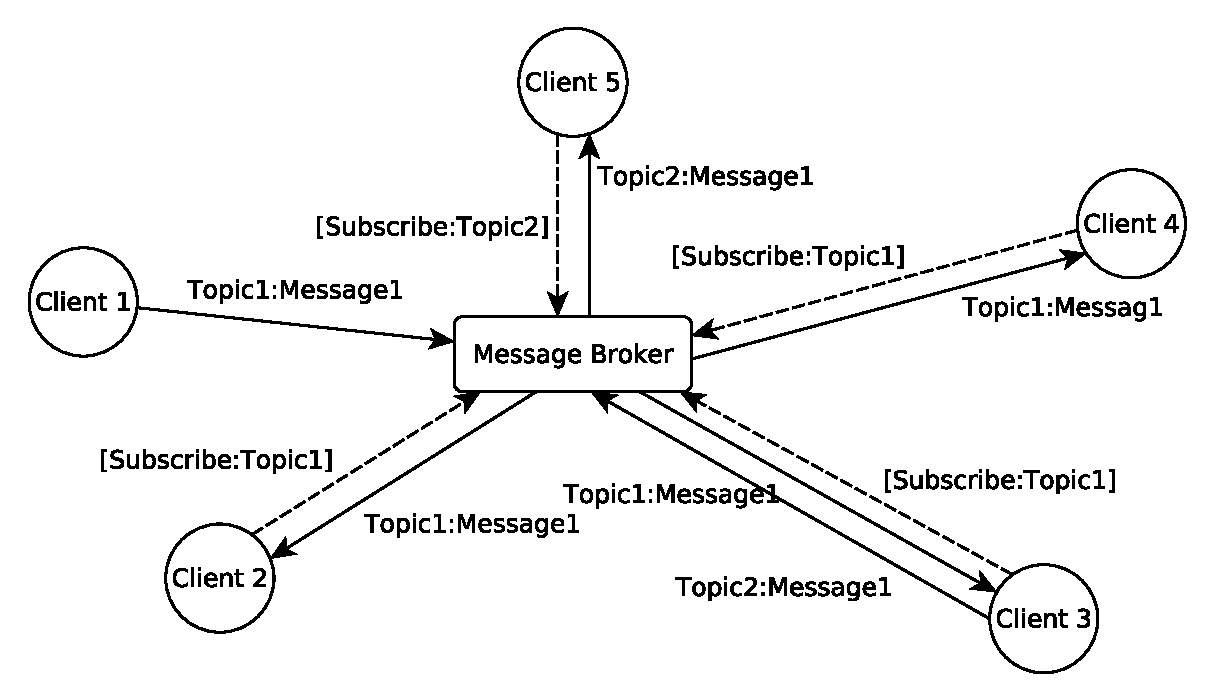
\includegraphics[width=0.95\linewidth]{MOM_BILD}
\caption{Schematische Darstellung der MOM-Architektur}
\label{fig:MOM_BILD}
\end{figure}


 Grundlage dieser Architektur ist das Advanced Messaging Queue Protocol (AMQP)\cite{wiki:AMQP}, welches die wichtigen Punkte Sicherheit, Zuverlässigkeit (\textit{Qualities of Service})und Kommunikationsverhalten spezifiziert. Aktuelle Implementierungen enthalten noch zusätzliche Funktionen zur Performancesteigerung und Ausfallsicherheit.


\section{Anforderungen und Evaluationskriterien}

\subsection{Hardwarevoraussetzungen}
Bei der Evaluation ist im IoT-Kontext zu beachten, dass nicht nur eine hohe Anzahl an Devices kommunizieren, sondern auch, dass diese sehr unterschiedliche Hardwarevoraussetzungen  mitbringen. 
\subsection{Clients}
%Systemvorraussetzungen -> Arduino
%C binding
Im IoT-Umfeld ist es üblich, dass Embedded Devices die Daten von verschiedenen Sensoren einsammeln und diese publizieren. Diese Systeme verfügen in der Regel nur über wenige Kilobyte Arbeitsspeicher und haben kein Betriebssystem. Um diese Systeme zu unterstützen, sollten die MOMs über ein C-Binding verfügen, welches in Umgebungen ohne Betriebssystem integriert werden kann und i.A. recourcenschonender ist als interpretierte Sprachen.

\subsection{Anbindung an BigData Server und Clouds}
Die von Sensoren generierten Daten werden im Allgemeinen auf Big Data Servern oder in Cloudlösungen abgelegt, die aus diesen Schlüsse ziehen. Hier sollte die Performance des Brokers keinen Flaschenhals des Systems darstellen, was neben Hardware- auch Softwareanforderungen stellt. So wäre z.B. eine Verteilung des Brokers auf mehrere Hardwareplattformen eine interessante Alternative. 

\section{Ausgewählte MOM-Implementierungen vorgestellt}
In diesem Abschnitt werden ausgewählte Implementierungen vorgestellt, welche alle unter nicht kommerziellen Lizenzen vertrieben werden und frei nutzbar sind. 
\subsection{Hinweis zur Bewertung}
Aufgrund des kurzen Zeitrahmens zur Ausarbeitung dieses Textes konnten nicht alle Entscheidungskriterien wissenschaftlich bewiesen (z.B. durch prototypische Implementierung oder Performancemessungen etc.) und hinreichend begründet werden und beruhen zum Teil auf einem ersten Eindruck und Gefühl. Diese Arbeit versteht sich eher als Basis für detailliertere Evaluationen. Das Fazit soll ebenfalls als  Vorschlag auf Basis der bisherigen Erkenntnisse als Diskussionsanregung dienen. 
\subsection{Übersicht über berücksichtigte Implementierungen}
Die folgenden Technologien wurden im Rahmen der Recherche berücksichtigt, jedoch nicht weiter verfolgt: 
\begin{itemize}
	\item Enduro/X: Interessante Ansätze (echtzeitfähig, POSIX Kernel Queues, ...) sehr junges Projekt und eine kleine Community
	%http://www.endurox.org/
	\item HornetQ: Sehr stark im High Performance Bereich angesiedelt
	%http://www.heise.de/developer/meldung/HornetQ-Neues-Messaging-System-von-JBoss-752869.html
	%http://hornetq.jboss.org/
	\item ZeroMQ: Läuft ohne Broker auf Basis von Berkley Sockets\cite{wiki:ZMQ}.
	%https://en.wikipedia.org/wiki/ZeroMQ
	\item StormMQ: Kein C-Binding, serviceorientiert, starker Fokus auf Sicherheit\cite{wiki:SMQ}. 
	%http://stormmq.com/
	\item NATS: Zu spät für ein detailiertes Review gefunden. Eher im high Performance Bereich angesiedelt\cite{DisMeQu}. 
	%https://en.wikipedia.org/wiki/NATS_Messaging
	\item MSMQ: Starke Abhängigkeiten zu Microsoft\cite{wiki:MsMessQueu}.
	\item Gearman: Keine aktive Entwicklung mehr\cite{wiki:GEAR}. 
	%https://en.wikipedia.org/wiki/Gearman
	\item Celery: Interessantes Konzept. Einstieg erscheint jedoch kompliziert\cite{wiki:CELERY}\cite{wiki:CWIKI}. 
	%http://www.celeryproject.org/docs-and-support/
\end{itemize}

\subsection{RabbitMQ}
Die erste der näher evaluierten Alternativen stellt RabbitMQ dar. RabbitMQ erweist sich den publizierten Informationen nach als sehr universell einsetzbar. Neben zahlreichen Aspekten zur Ausfallsicherheit und Hochverfügbarkeit verfügt es ebenfalls über ein Management Plugin im Broker, welches Konfiguration, Monitoring und Debugging vereinfacht\cite{WHATRMQ}. Des weiteren verfügt RabbitMQ über ein C-Binding, über dessen Kompatibilität zu Embedded Systems kann aktuell jedoch keine Aussage getroffen werden\cite{RMQEMB}\cite{RMQ_IOT}. Ein positiver Aspekt ist ebenfalls, dass RabitMQ seit Jahren aktiv weiterentwickelt wird und über eine groß Community verfügt. 
%C_binding 
\subsection{MQTT}
Traut man Internetnachrichtendiensten oder schaut man auf die Agenden von Developertalks, so bekommt man den Eindruck, dass sich MQTT als Standardprotokoll im IoT Umfeld etabliert hat\cite{UNDERPROT}\cite{FIVETHINGS}. Der Hauptgrund dafür sind vor allem die sehr leichtgewichtigen Clientimplementierungen, welche auf den kleinsten SoCs lauffähig sind.\cite{wiki:MQTT} Auch der Broker ist eher auf Einfachheit optimiert und verzichtet beispielsweise auf eine Autorisierung, um die Nachrichtenlänge möglichst kurz zu halten\cite{MQTTSEC}. Außerdem wurde auf Replikationsoptionen, Clustering und Fehlerbehandlungen verzichtet. Vermutlich ist die maximale Performance des MQTT Brokers den anderen Technologien ebenfalls unterlegen. Diese Einfachheit ermöglicht jedoch auch eine zielstrebige Implementierung von Prototypen\cite{KOMQTT}\cite{KOMAPPIN}. 
%C binding 
%Embedded Devices kompatibel
%Limitierungen im HighPerformance bereich

\subsection{Apache ActiveMQ}
Die Hauptvorteile von ActiveMQ bestehen in der Möglichkeit, ein Netz aus Brokern zu betreiben, in dem Clients sich zu einem beliebigen Broker verbinden. Fällt der Broker aus, wird automatisch ein Reconnect auf einem anderen Brocker durchgeführt. Das Routing zwischen den Endpunkt findet dabei vollkommen transparent zum Client statt. Replikation von Brokern wird ebenfalls unterstützt. Dadurch wird ActiveMQ hohen Anforderungen an Performance und Ausfallsicherheit gerecht. Für die Clientintegration stehen zahlreiche Bindings zur Verfügung, welche laut Apache jedoch primär darauf abzielen, legacy Code von Enterpriseapplications zu in neue MOM-Umgebungen integrieren. Auch ActiveMQ wird aktuell noch weiterentwickelt und verfügt über eine ausführliche Dokumentation.\cite{wiki:AAMQ}

\subsection{Apache Kafka}
Apache Kafka stellt mit einem anderen Konzept eine Alternative zu den zuvor vorgestellten Technologien dar. Kafka stellt primär ein Software Paket zur Verarbeitung von Datenströmen dar, welches hoch skalierbar ist und verteilt operieren kann und somit hervorragend im BigData Bereich einsetzbar ist\cite{wiki:AKAFKA}\footnote{Kafka ist also streng genommen keine Message Oriented Middleware. Da es sich aber u.U. um eine für das Projekt interessante Technologie handelt, soll sie hier trotzdem Beachtung finden.}. Kafka ist in der Lage, große Nachrichtenvolumen durch Load Balancing und Clustering deutlich schneller zu verarbeiten, als eine MOM Lösung, kann jedoch nicht ohne eines der o.g. MOMs als Datenquelle eingesetzt werden und wäre daher eher Teil einer hybriden Lösung, wie in \ref{test} beschrieben. Kafka soll leicht installierbar sein und verfügt über eine unfangreiche Dokumentation\cite{AKW}. 

\subsection{Hybride Lösungen}\label{test}
%http://blog.airasoul.io/the-internet-of-things-with-rabbitmq-node-js-mqtt-and-amqp/
Wie bereits in der Einführung beschrieben, kommen im Bereich IoT-Systeme mit sehr unterschiedlichen Hardwarevorraussetzungen zum Einsatz. Dies macht eine hybride Lösung aus mehreren Middlewaretechnologien interessant. 

Zum einen wäre eine Zwei-Stufen-Lösung denkbar, in der ein oder mehrere Message Broker ein Kafka BigData System mit Daten versorgen, welches diese aufbereitet und in einer Cloud ablegt. Hierbei sollte im aktuellen Projekt jedoch Implementierungsaufwand und Nutzen abgewogen werden. 

Zum anderen existieren Schnittstellen zwischen den vorgestellten Systemen, die es möglich machen, die Vorteile der jeweiligen Systeme zu nutzen. Mehrwert und Funktionalität sollten aber auch hier genau evaluiert werden.

% use section* for acknowledgement
\section{Fazit in Bezug auf das konkrete Projekt}
Zusammenfassend kann man sagen, dass jede der vorgestellten Message Oriented Middleware Implementierungen, RabbitMQ, MQTT und ApacheMQ, prinzipiell die gestellten Anforderungen erfüllt\cite{ExplMessBrok}. Geht man weiter ins Detail, offenbaren sich Unterschiede, die für das Projekt relevant sein können. Daher sollte die Entscheidung welche Technologie eingesetzt wird, auf Basis der Embedded Devices, die verwendet werden und des erwarteten Nachrichtenvolumens im gesamten Netzwerk getroffen werden. Außerdem sind implementierungsspezifische Besonderheiten der jeweiligen MOM noch nicht bekannt. Auch eine Implementierung, die hier nicht näher betrachtet wurde, wie EnduroX oder NATS, wäre prinzipiell für den Einsatz im Projekt denkbar.  Ein weiterer wichtiger Entscheidungspunkt ist inwieweit Data Streaming Architecturs und Clouddienste zum Einsatz kommen sollen und diese selbst bereit gestellt werden sollen. Für diese Anforderung bietet Apache Kafka ein mächtiges Werkzeug.

\section{Die nächsten Schritte}
Als nächsten Schritte sollten nun zum einen die Anforderungen an die Message Oriented Middleware auf Basis der genauen Projektbeschreibung ausgearbeitet werden. Zum anderen sollte ein beispielhaftes Setup und eine Referenzimplementierung für die in Frage kommenden Systeme erfolgen, um Limitierungen und Schwierigkeiten möglichst frühzeitig zu erkennen.
\citeschund{banavar1999case}
\cite{estrada2015comparing}


% if have a single appendix:
%\appendix[Proof of the Zonklar Equations]
% or
%\appendix  % for no appendix heading
% do not use \section anymore after \appendix, only \section*
% is possibly needed

% use appendices with more than one appendix
% then use \section to start each appendix
% you must declare a \section before using any
% \subsection or using \label (\appendices by itself
% starts a section numbered zero.)
%

\appendices


% Can use something like this to put references on a page
% by themselves when using endfloat and the captionsoff option.
\ifCLASSOPTIONcaptionsoff
  \newpage
\fi



% trigger a \newpage just before the given reference
% number - used to balance the columns on the last page
% adjust value as needed - may need to be readjusted if
% the document is modified later
%\IEEEtriggeratref{8}
% The "triggered" command can be changed if desired:
%\IEEEtriggercmd{\enlargethispage{-5in}}

% references section

% can use a bibliography generated by BibTeX as a .bbl file
% BibTeX documentation can be easily obtained at:
% http://www.ctan.org/tex-archive/biblio/bibtex/contrib/doc/
% The IEEEtran BibTeX style support page is at:
% http://www.michaelshell.org/tex/ieeetran/bibtex/
%\bibliographystyle{IEEEtran}
% argument is your BibTeX string definitions and bibliography database(s)
%\bibliography{IEEEabrv,../bib/paper}
%
% <OR> manually copy in the resultant .bbl file
% set second argument of \begin to the number of references
% (used to reserve space for the reference number labels box)
\nocite{*}
\nociteschund{*}
\renewcommand\refname{Quellen}
\bibliography{Quellen} 

%%%%%%%%%%%%%%%%%%%%%%%%%%%%%%
% Achtung unbedingt mit 
% bibtex main 
% und
% bibtex schund 
% kompilieren
%%%%%%%%%%%%%%%%%%%%%%%%%%

\bibliographystyleschund{ieeetr}
\bibliographyschund{Quellen2}


% biography section
% 
% If you have an EPS/PDF photo (graphicx package needed) extra braces are
% needed around the contents of the optional argument to biography to prevent
% the LaTeX parser from getting confused when it sees the complicated
% \includegraphics command within an optional argument. (You could create
% your own custom macro containing the \includegraphics command to make things
% simpler here.)
%\begin{biography}[{\includegraphics[width=1in,height=1.25in,clip,keepaspectratio]{mshell}}]{Michael Shell}
% or if you just want to reserve a space for a photo:



% You can push biographies down or up by placing
% a \vfill before or after them. The appropriate
% use of \vfill depends on what kind of text is
% on the last page and whether or not the columns
% are being equalized.

%\vfill

% Can be used to pull up biographies so that the bottom of the last one
% is flush with the other column.
%\enlargethispage{-5in}




% that's all folks
\end{document}


\grid
